\section{Method}
	We implement the Fast Marching Method (FMM) for solving the Eikonal equation in 3D cartesian coordinates (Figure \ref{fig:coordinate_axes}) using a mixed- (first- and second-) order update scheme.
	\par
	
	\begin{figure}
	\centering
	\begin{tikzpicture}[axis/.style={thin, black, ->, >=stealth'}]
		\draw[axis] (0,0) -- (0,2) node [above, black] {\scriptsize -Y};
		\draw[axis] (0,0) -- (0,-2) node [below, black] {\scriptsize +Y};
		\draw[axis] (0,0) -- (2,0) node [right, black] {\scriptsize +X};
		\draw[axis] (0,0) -- (-2,0) node [left, black] {\scriptsize -X};
		\draw[axis] (0,0) -- (45:2) node [right, black] {\scriptsize +Z};
		\draw[axis] (0,0) -- (225:2) node [left, black] {\scriptsize -Z};
	\end{tikzpicture}
	\caption{Convention adopted throughout this article for the orientation of Cartesian coordinate axes}
	\label{fig:coordinate_axes}
\end{figure}

	\subsection{Statement of the problem}
		Consider a curve $\Gamma\left(t\right)$ that propagates perpendicular to itself with velocity $v$, and let $u\left(\mathbf{r}\right)$ be the time that the front crosses the point with position vector $\mathbf{r}$. Further, let the propagation velocity also be a function of space and assume that it is strictly positive everywhere, i.e., $v\left(\mathbf{r}\right) > 0 \ \forall\ \mathbf{r}$. The relationship between $u\left(\mathbf{r}\right)$ and $v\left(\mathbf{r}\right)$ is given by the Eikonal equation,
		
		\begin{equation}
			\label{eqn:eikonal}
			\left|\nabla u\left(\mathbf{r}\right)\right| = \frac{1}{v\left(\mathbf{r}\right)},
		\end{equation}
		
		\noindent and the curve $\Gamma\left(t\right)$ is given by $\Gamma\left(t\right) = \left\{\mathbf{r}\ \mid\ u\left(\mathbf{r}\right) = t\right\}$. $\Gamma\left(t\right)$ then is the $t$ level-set of $u$ and the evolution of $\Gamma$ can be tracked by solving Eqn (\ref{eqn:eikonal}) for $u\left(\mathbf{r}\right)$ if $v\left(\mathbf{r}\right)$ is known.
		\par
		
		The problem is to solve Eqn (\ref{eqn:eikonal}) for $u\left(\mathbf{r}\right)$, given $\Gamma\left(t=0\right)$ and $v\left(\mathbf{r}\right)$.
	
	\subsection{Solution}
		\citeA{Sethian1996} proposed an efficient numerical method---the Fast Marching Method (FMM)---for approximating a solution to Eqn (\ref{eqn:eikonal}), subject to an entropy condition: \textit{$\Gamma\left(t\right)$ can only cross any point once.} Imposing this entropy condition implies that the solution obtained comprises only first arrivals; $\Gamma\left(t\right)$ propagates along the shortest (in terms of time) possible path between any two points.
		\par
		
		Briefly, the FMM, as implemented here, is as follows. The reader is referred to the original paper \cite{Sethian1996} for a detailed explanation.
		\par
		
	\subsection{The Fast Marching Method}
		Express Eqn (\ref{eqn:eikonal}) in discrete Cartesian coordinates:
		
		\begin{equation}
			\label{eqn:discrete_eikonal_index_form}
			\left|\nabla u_{ijk}\right| = \frac{1}{v_{ijk}}.
		\end{equation}
	
		\noindent where
	
		\begin{equation}
			f_{ijk} \equiv f\left(i\Delta x, j\Delta y, k\Delta z\right),
		\end{equation}
		
		\noindent $i, j, k \in \mathbb{Z}$, and $\Delta x, \Delta y, \Delta z$ are the discretization intervals along the x, y, and z axis, respectively.
		\par
		
		Now substitute the entropy-satisfying approximation to the gradient from \citeA{Rouy1992}
		
		\begin{equation}
			\label{eqn:gradient_approximation}
			\left|\nabla u_{ijk}\right| ^2 \approx 
			\sum_{\xi \in \left[x, y, z\right]} max\left(D^{-\xi}_{ijk}, -D^{+\xi}_{ijk}, 0 \right)^2
		\end{equation}
		
		\noindent into Eqn(\ref{eqn:discrete_eikonal_index_form}) to get
		
		\begin{equation}
			\label{eqn:discrete_eikonal_approximation}
			\sum_{\xi \in \left[x, y, z\right]} max\left(D^{-\xi}_{ijk}, -D^{+\xi}_{ijk}, 0 \right)^2 - \frac{1}{v^2_{ijk}} \approx 0
		\end{equation}
		
		\noindent where $D^{-\xi}_{ijk}$ and $D^{+\xi}_{ijk}$ represent backward and forward finite-difference approximations to the derivative of $u_{ijk}$ along the $\xi$ axis, respectively.
		\par
		
		Eqn (\ref{eqn:discrete_eikonal_approximation}) has an \textit{upwind} difference structure---a causality relationship implying that the value of $u_{ijk}$ is fully determined by neighbouring values of $u_{lmn}$ where $u_{lmn} < u_{ijk}$. With this formulation, information only propagates \textit{downwind}, and $u_{ijk}$ is said to be downwind of $u_{lmn}$ if $u_{lmn} < u_{ijk}$. The FMM leverages this upwind structure in the following update scheme (Algorithm \ref{alg:fmm_update}), which builds the solution of $u$ by iteratively solving Eqn (\ref{eqn:discrete_eikonal_approximation}) for unknown values of $u$ in a narrow band separating upwind nodes from downwind based on the values of their known upwind neighbours.
		\par
		
		\begin{algorithm}
			\SetAlgoLined
			\ForEach{
				\text{\normalfont Node in grid}
			}{
				Tag node as \textit{Far/Downwind}\;
			}
			\ForEach{
				$Node\ \in\ \Gamma\left(t=0\right)$
			}{
				Remove \textit{Far/Downwind} tag from node\;
				Add node to \textit{Close/Narrow Band} list\;
				$u_{ijk} \gets 0$\;
			}
			\While{
				\text{\normalfont{length}}$(\textit{Close/Narrow Band}) > 0$
			}{
				$Trial \gets\ $node in \textit{Close/Narrow Band} with smallest value of $u$\;
				Remove \textit{Trial} node from \textit{Close/Narrow Band}\;
				Tag \textit{Trial} node as \textit{Alive/Upwind}\;
				\ForEach{
					\text{\normalfont Neighbour of} Trial
				}{
					\If{
						\text{\normalfont Neighbour is} \textit{Far/Downwind}
					}{
						Remove \textit{Far/Downwind} tag from node\;
						Add node to \textit{Close/Narrow Band} list\;
					}
					Recompute value of $u$ for \textit{Neighbour} by solving Eqn (\ref{eqn:discrete_eikonal_approximation})\;
				}
			}
			\caption{FMM update scheme for solving the Eikonal equation.}
			\label{alg:fmm_update}
		\end{algorithm}

		\begin{figure}
	\centering
	\makebox[\textwidth][c]{
		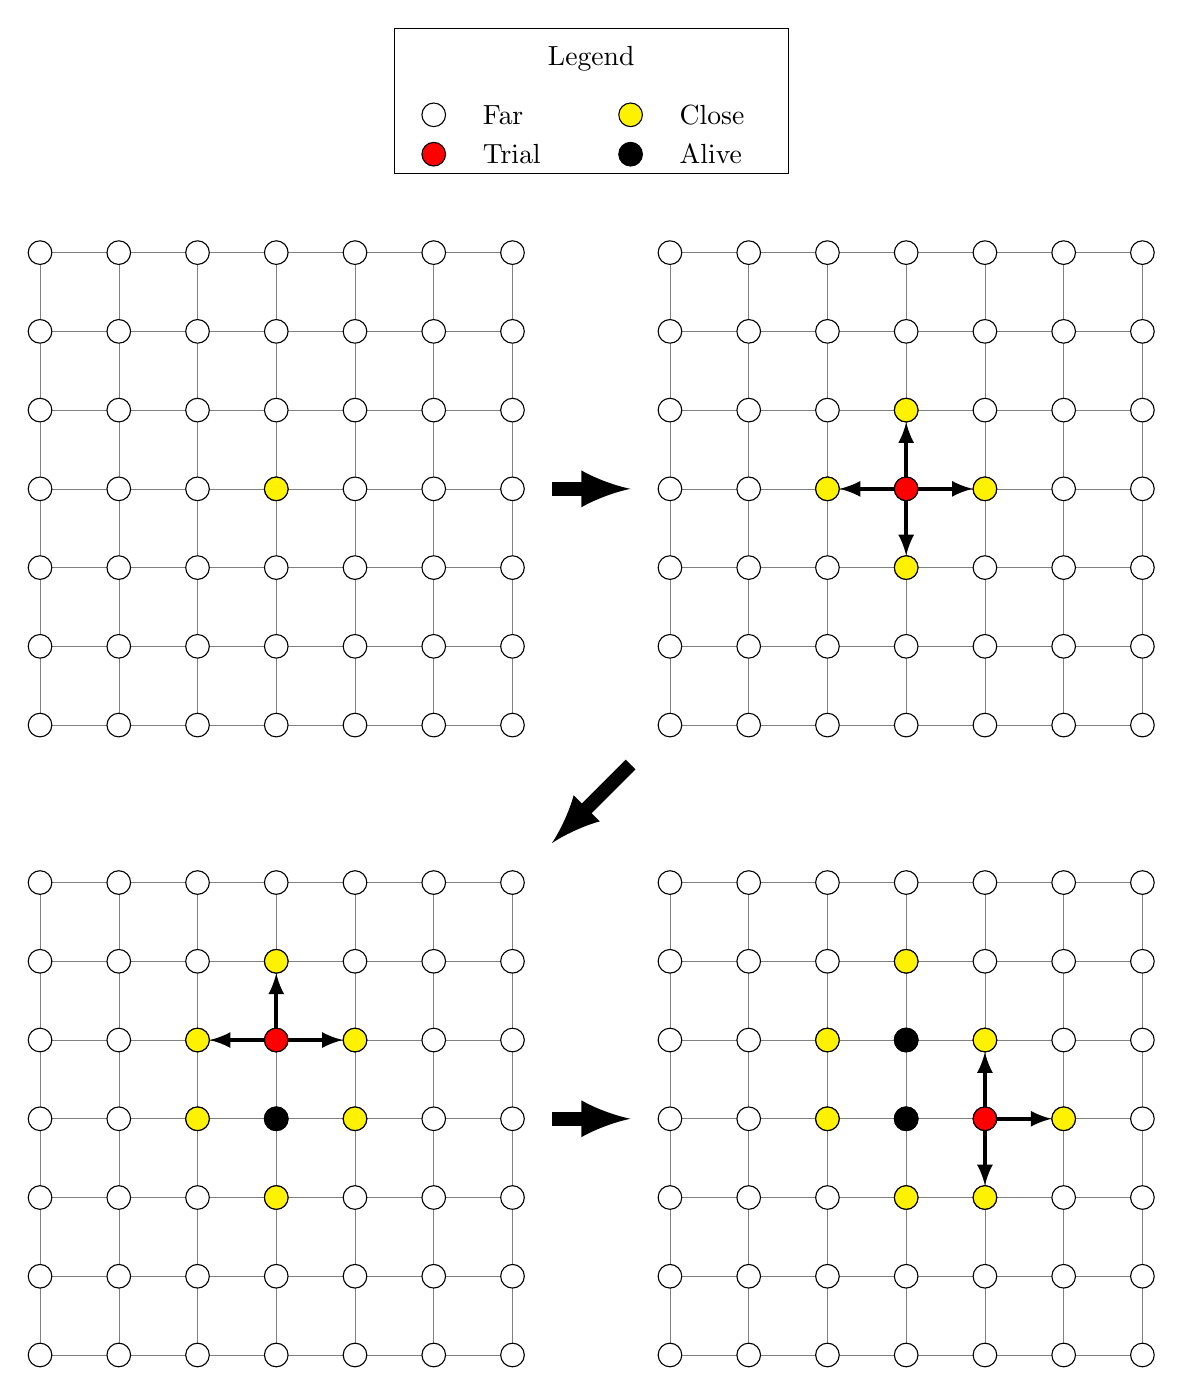
\begin{tikzpicture}[axis/.style={thin, black, ->, >=stealth'}]
			
			\def \radius{0.15}
			\def \cfar{white}
			\def \cclose{yellow}
			\def \ctrial{red}
			\def \calive{black}
			
			\draw (4.5, 15) rectangle (9.5, 16.85);
			\node[align=left,anchor=north] at (7, 16.75) {Legend};
			\filldraw[fill=\cfar]             (5,  15.75) circle (\radius);
			\node[align=left,anchor=west] at  (5.5,15.75) {Far};	
			\filldraw[fill=\cclose]           (7.5,  15.75) circle (\radius);
			\node[align=left,anchor=west] at  (8,    15.75) {Close};
			
			\filldraw[fill=\ctrial]           (5,  15.25) circle (\radius);
			\node[align=left,anchor=west] at  (5.5,15.25) {Trial};
			
			\filldraw[fill=\calive]           (7.5,15.25) circle (\radius);
			\node[align=left,anchor=west] at  (8,  15.25) {Alive};
	
			% GRID A
			\def \xmin{0}
			\def \xmax{6}
			\def \ymin{8}
			\def \ymax{14}
			\draw[step=1cm,gray,very thin] (\xmin, \ymin) grid (\xmax, \ymax);
			\foreach \ix in {\xmin,...,\xmax}{
				\foreach \iy in {\ymin,...,\ymax}{
					\filldraw[fill=\cfar] (\ix,\iy) circle (\radius);
				}
			}
			\filldraw[fill=\cclose] (\xmin+3,\ymin+3) circle (\radius);
			
			\draw[-latex,line width=5pt] (\xmax+0.5, \ymin+3) -- (\xmax+1.5, \ymin+3);
			
			% GRID B
			\def \xmin{8}
			\def \xmax{14}
			\def \ymin{8}
			\def \ymax{14}
			\draw[step=1cm,gray,very thin] (\xmin, \ymin) grid (\xmax, \ymax);
			\foreach \ix in {\xmin,...,\xmax}{
				\foreach \iy in {\ymin,...,\ymax}{
					\filldraw[fill=\cfar] (\ix,\iy) circle (\radius);
				}
			}
			\filldraw[fill=\ctrial] (\xmin+3,\ymin+3) circle (\radius);
			\filldraw[fill=\cclose] (\xmin+3,\ymin+4) circle (\radius);
			\filldraw[fill=\cclose] (\xmin+3,\ymin+2) circle (\radius);
			\filldraw[fill=\cclose] (\xmin+4,\ymin+3) circle (\radius);
			\filldraw[fill=\cclose] (\xmin+2,\ymin+3) circle (\radius);
	
			\draw[-latex,ultra thick] (\xmin+3, \ymin+3+\radius) -- (\xmin+3, \ymin+4-\radius);
			\draw[-latex,ultra thick] (\xmin+3, \ymin+3-\radius) -- (\xmin+3, \ymin+2+\radius);
			\draw[-latex,ultra thick] (\xmin+3+\radius, \ymin+3) -- (\xmin+4-\radius, \ymin+3);
			\draw[-latex,ultra thick] (\xmin+3-\radius, \ymin+3) -- (\xmin+2+\radius, \ymin+3);
			
			\draw[-latex,line width=5pt] (\xmin-0.5, \ymin-0.5) -- (\xmin-1.5, \ymin-1.5);
			
			% GRID C
			\def \xmin{0}
			\def \xmax{6}
			\def \ymin{0}
			\def \ymax{6}
			\draw[step=1cm,gray,very thin] (\xmin, \ymin) grid (\xmax, \ymax);
			\foreach \ix in {\xmin,...,\xmax}{
				\foreach \iy in {\ymin,...,\ymax}{
					\filldraw[fill=\cfar] (\ix,\iy) circle (\radius);
				}
			}
			\filldraw[fill=\calive] (\xmin+3,\ymin+3) circle (\radius);
			\filldraw[fill=\ctrial] (\xmin+3,\ymin+4) circle (\radius);
			\filldraw[fill=\cclose] (\xmin+3,\ymin+2) circle (\radius);
			\filldraw[fill=\cclose] (\xmin+4,\ymin+3) circle (\radius);
			\filldraw[fill=\cclose] (\xmin+2,\ymin+3) circle (\radius);
			\filldraw[fill=\cclose] (\xmin+3,\ymin+5) circle (\radius);
			\filldraw[fill=\cclose] (\xmin+4,\ymin+4) circle (\radius);
			\filldraw[fill=\cclose] (\xmin+2,\ymin+4) circle (\radius);
			
			\draw[-latex,ultra thick] (\xmin+3, \ymin+4+\radius) -- (\xmin+3, \ymin+5-\radius);
			\draw[-latex,ultra thick] (\xmin+3+\radius, \ymin+4) -- (\xmin+4-\radius, \ymin+4);
			\draw[-latex,ultra thick] (\xmin+3-\radius, \ymin+4) -- (\xmin+2+\radius, \ymin+4);
			
			\draw[-latex,line width=5pt] (\xmax+0.5, \ymin+3) -- (\xmax+1.5, \ymin+3);
			
			% GRID D
			\def \xmin{8}
			\def \xmax{14}
			\def \ymin{0}
			\def \ymax{6}
			\draw[step=1cm,gray,very thin] (\xmin, \ymin) grid (\xmax, \ymax);
			\foreach \ix in {\xmin,...,\xmax}{
				\foreach \iy in {\ymin,...,\ymax}{
					\filldraw[fill=\cfar] (\ix,\iy) circle (\radius);
				}
			}
			\filldraw[fill=\calive] (\xmin+3,\ymin+3) circle (\radius);
			\filldraw[fill=\calive] (\xmin+3,\ymin+4) circle (\radius);
			\filldraw[fill=\cclose] (\xmin+3,\ymin+2) circle (\radius);
			\filldraw[fill=\ctrial] (\xmin+4,\ymin+3) circle (\radius);
			\filldraw[fill=\cclose] (\xmin+2,\ymin+3) circle (\radius);
			\filldraw[fill=\cclose] (\xmin+3,\ymin+5) circle (\radius);
			\filldraw[fill=\cclose] (\xmin+4,\ymin+4) circle (\radius);
			\filldraw[fill=\cclose] (\xmin+2,\ymin+4) circle (\radius);
			\filldraw[fill=\cclose] (\xmin+5,\ymin+3) circle (\radius);
			\filldraw[fill=\cclose] (\xmin+4,\ymin+2) circle (\radius);
			
			\draw[-latex,ultra thick] (\xmin+4, \ymin+3+\radius) -- (\xmin+4, \ymin+4-\radius);
			\draw[-latex,ultra thick] (\xmin+4+\radius, \ymin+3) -- (\xmin+5-\radius, \ymin+3);
			\draw[-latex,ultra thick] (\xmin+4, \ymin+3-\radius) -- (\xmin+4, \ymin+2+\radius);
			
	
		\end{tikzpicture}
	}
	\caption{A 2D illustration of the update scheme (Algorithm \ref{alg:fmm_update}) used by the FMM}
	\label{fig:fmm_update}
\end{figure}

	\subsection{Accuracy of the FMM}
		The accuracy of the FMM depends partially on the order of the finite-difference operators used where generic finite differences are specified in Eqn (\ref{eqn:discrete_eikonal_approximation}). The simplest and least-accurate scheme uses only first-order operators:
		
		\begin{equation}
			D^{-x}_{ijk} = D^{-x^1}_{ijk} \equiv \frac{u_{ijk}-u_{i-1jk}}{\Delta x},
		\end{equation}
		
		\begin{equation}
			D^{+x}_{ijk} = D^{+x^1}_{ijk} \equiv \frac{u_{i+1jk}-u_{ijk}}{\Delta x},
		\end{equation}
		
		\noindent and similar definitions in $y$ and $z$. More accurate approximations, however, can be obtained by using higher-order operators, e.g.,
		\begin{equation}
			D^{-x}_{ijk} = D^{-x^2}_{ijk} \equiv \frac{u_{i+2jk}-4u_{i+1jk}+3u_{ijk}}{2\Delta x},
		\end{equation}
		
		\begin{equation}
			D^{+x}_{ijk} = D^{+x^2}_{ijk} \equiv -\frac{u_{i-2jk}-4u_{i-1jk}+3u_{ijk}}{2\Delta x},
		\end{equation}
		and similar definitions in $y$ and $z$.
		
		Following \citeA{Sethian1999a} we compute values of $u_{ijk}$ using a second-order update when sufficient upwind data exists. The algorithm used for choosing the update order is most concisely expressed as pseduo-code (Algorithm \ref{alg:update_order}).
		
		\begin{algorithm}
			\SetAlgoLined
			\uIf{
				$u_{i-2jk}, u_{i-1jk}\ \in$ Alive/Upwind \text{\normalfont\textbf{AND}}  $u_{i-2jk} < u_{i-1jk} < u_{ijk}$
			}{
				$D^{-x}_{ijk} \gets D^{-x^2}_{ijk}$\;
			}
			\uElseIf{
				$u_{i-1jk}\ \in$ Alive/Upwind \text{\normalfont\textbf{AND}}  $u_{i-1jk} < u_{ijk}$
			}{
				$D^{-x}_{ijk} \gets D^{-x^1}_{ijk}$\;
			}
			\uElse{
				$D^{-x}_{ijk} \gets 0$\;
			}
			\caption{Algorithm for choosing the order for $D^{-x}_{ijk}$. Similar algorithms are implemented for $D^{+x}_{ijk}$, $D^{\pm y}_{ijk}$, and $D^{\pm z}_{ijk}$}.
			\label{alg:update_order}
		\end{algorithm}